\begin{center}
	\begin{tikzpicture}[node distance =  2.75cm,auto,fontscale=0.01]
	\linespread{1}
	\visible<1-10>{\node [rectangle,minimum width=4.4cm,minimum height =4.2cm,anchor=center, 
		path picture= {\node at (path picture bounding box.center){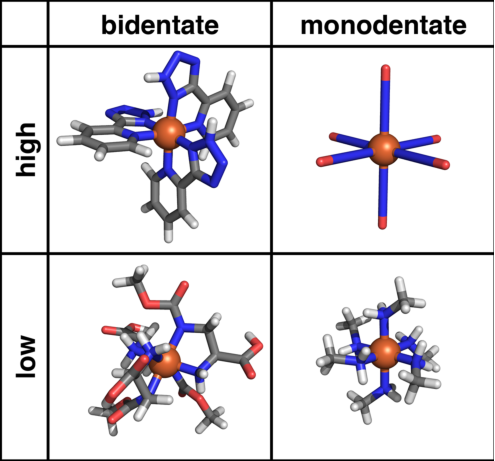
\includegraphics[width=4.5cm]{representations/images/fig10.pdf}{}};}](ff) at (0,0){};
		\node[rectangle,text=black,draw=blue,thick,fill = gray, fill opacity=0.25,text opacity= 1] (hm) at (1.75,1.4){\tiny 4.0V};
		\node[rectangle,text=black,draw=blue,thick,fill = gray, fill opacity=0.25,text opacity= 1] (hb) at (-1.4,1.4){\tiny 2.0V};
		\node[rectangle,text=black,draw=blue,thick,fill = gray, fill opacity=0.25,text opacity= 1] (hl) at (1.75,-0.5){\tiny 1.0V};
		\node[rectangle,text=black,draw=red,thick,fill = gray, fill opacity=0.25,text opacity= 1] (hl) at (-1.4,-0.5){\tiny -0.3V};}
	%%%%%%%%%%%%%%%%%%%%%%%%%%%%%%%%%%%%%%%%%%%%%%%
	\visible<2-8>{\node[](labq) at (0,-2.35) {\small How can we account for the difference?};}
	%%%%%%%%%%%%%%%%%%%%%%%%%%%%%%%%%%%%%%%%%%%%%%%
	\visible<3->{\node [rectangle,text width = 4.85cm,anchor=north] (tb) at (-5,2) { \begin{small}Could correlate with:
			\begin{itemize}
			\visible<4->{\item{$\chi$ (ANN paper)}}
			\visible<5->{\item{$Z$ (Coulomb matrix)}}
			\visible<6->{\item{$T$ (topology $\sim$ Randi\'{c})}}
			\visible<7->{\item{$I$ (count/size)}}
			\end{itemize}%
			\visible<8->{Can use \emph{autocorrelation} \mbox{functions} to describe how ligand atoms are connected}%
			\end{small}};}  
	%%%%%%%%%%%%%%%%%%%%%%%%%%%%%%%%%%%%
	\visible<9>{\node[rectangle,minimum width=4.4cm,minimum height =4.3cm,anchor=center,fill=white,text width = 4.5cm](ff) at (0,0){$\begin{aligned}
			\eta_{i,0} &=  p_i p_i  \\
			\eta_{i,k} &= \sum_{i\neq j} p_i p_j \delta(d_{i,j} -  d_k ), \:\: k\neq 0\\
			\text{AC}_k &=\sum_{i}\eta_{i,k}
			\end{aligned}$\\
			{4 properties, $k\in \left[0,5\right]$ $\implies$ 28 variables.}\\ {\color{red} How to choose?}};}
	%%%%%%%%%%%%%%%%%%%%%%%%%%%%%%%%%%%%%%%%%%%%%%%%%%%%%%%%%%%%%%%%%%
	
	\visible<10->{\node [rectangle,,minimum width=6cm,minimum height =6cm,fill=white,text width = 6cm,anchor=center,path picture= {\node at (path picture bounding box.center){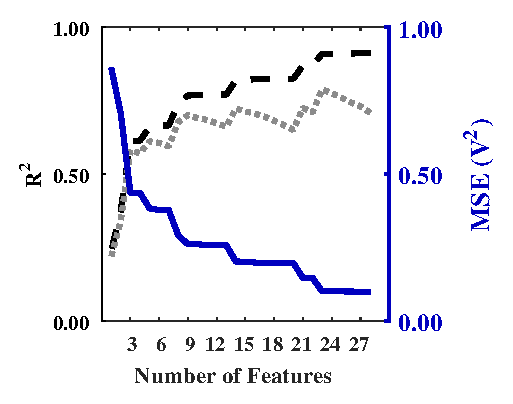
\includegraphics[width=6cm]{representations/figures/rmse}{}};}] (tb) at (-5.0,-0.15) {};}
	\visible<11->{\node [rectangle,,minimum width=4.5cm,minimum height =5cm,text width = 4.85cm,anchor=center,path picture= {\node at (path picture bounding box.center){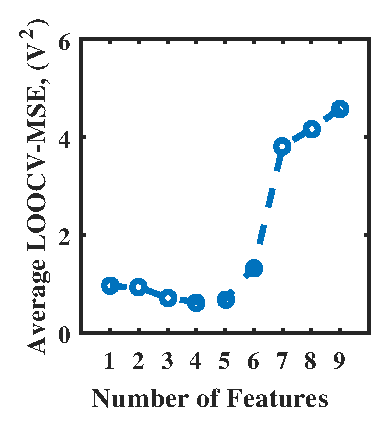
\includegraphics[width=4.5cm]{representationsfigures/cv}{}};}] (tb) at (0,-0.15) {};}
	%%%%%%%%%%%%%%%%%%%%%%%%%%%%%%%%%%%%%%%%%%%%%%%%%%%%%%%%%%%%%%%%%%%%%%%
	
	\end{tikzpicture}
\end{center}

